\section{Veranschaulichung mit Kripke-Modellen}
\label{Kripke-Modelle}
Das Kripke-Modell eines verteilten Systems mit kleiner Anzahl Prozesse kann intuitiv als Graph dargestellt werden (vgl. \cite{kshemkalyani2011distributed} S. 285 ff.). Dabei entspricht jeder Systemzustand $s\in S$ einem Knoten, der mit der Belegung der atomaren Aussagen $\Phi$ beschriftet wird. Eine Kante wird zwischen zwei Knoten gezeichnet, wenn es mindestens einen Prozess gibt, der die repräsentierten Systemzustände nicht voneinander unterscheiden kann. Sie wird mit den Nummern aller Prozesse beschriftet für die dies gilt.
Der Graph ist dementsprechend bidirektional und reflexiv.\\
Mit Hilfe der Erreichbarkeit können die Definitionen zu den \textit{jeder-weiß}- und den gemeinsames Wissen-Operator auf diese Graphen übertragen werden:
\begin{itemize}
	\item Ein Zustand t kann vom Zustand s in k Schritten erreicht werden (ist k-erreichbar), wenn es eine Folge von Zuständen $s_0,s_1,...,s_k$ gibt, wobei $s_0 = s$, $s_k = t$ mit einem Zustand $P_i$ zu jedem $j\in [ 0,k-1 ]$, sodass $(s_j,s_{j+1})\in \mathcal{K}_i$
	\item Ein Zustand t ist vom Zustand s aus erreichbar, wenn es ein beliebiges $k \ge 0$\footnote{\label{note1}In \cite{kshemkalyani2011distributed} S. 286 wird dies für ein $k > 0$ definiert. Zum Ende des Kapitels wird auf den Unterschied eingegangen.} gibt, sodass t von s in k Schritten erreicht werden kann.
\end{itemize}
Man kann also direkt am Graphen erkennen, welche Zustände von einem anderen k-erreichbar sind, indem man alle Wege verfolgt, die sich mit k Kanten bilden lassen.
Generell erreichbar ist ein Zustand, wenn es eine ununterbrochene Verbindung zu ihm gibt.
Daraus ergeben sich für den \textit{jeder-weiß}- und den gemeinsames Wissen-Operator folgende Definitionen:
\begin{itemize}
	\item (M,s) $\vDash E^{k}(\phi)$, genau dann wenn (M,t) $\vDash \phi$ für alle Zustände t gilt, die vom Zustand s in k (oder weniger)\footnote{\label{note2}In \cite{kshemkalyani2011distributed} S. 286 fehlt dieser Zusatz. Zum Ende des Kapitels wird auf den Unterschied eingegangen.} Schritten erreichbar sind.
	\item (M,s) $\vDash C(\phi)$, genau dann wenn (M,t) $\vDash \phi$ für alle Zustände t gilt, die vom Zustand s erreichbar sind.
\end{itemize}
Um im Graphen zu erkennen, ob $E^{k}(\phi)$ in einem Zustand s gilt, muss man dementsprechend überprüfen, ob $\phi$ in allen Zuständen wahr ist, die sich in k oder weniger Schritten erreichen lassen. 
Warum diese Definitionen mit den vorherigen übereinstimmen werden wir anhand mehrerer Beispiele im Folgenden erkennen.

\subsection{Kripke-Modelle zum \textit{cheating husbands}-Rätsel}
Die aufgestellten Definitionen können mit Hilfe des \textit{cheating husbands}-Rätsels veranschaulicht werden.
Für den Fall, dass es drei Ehepaare in Atlantis gibt, lässt sich die Situation noch dreidimensional darstellen.
In Abbildung \ref{ausgang} betrachten wir zunächst die Ausgangssituation noch bevor die Königin ihre Ansprache gehalten hat.
Ein Zustand (0,0,1) im Graphen bedeutet, dass der Ehemann des dritten Ehepaares untreu war, während die anderen beiden treu waren.

\begin{figure}
\centering
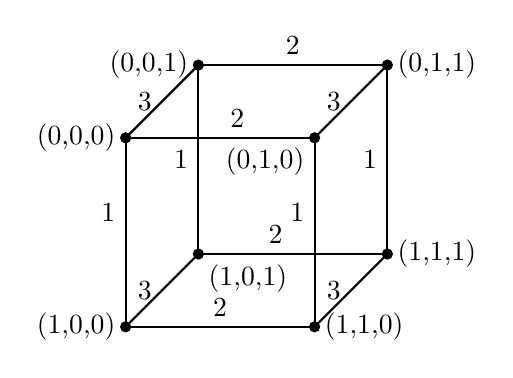
\begin{tikzpicture}[thick,scale=0.2]
\coordinate[label={180:\text{(1,0,0)}}] (UVL) at (0,0,12);
\coordinate[label={0:\text{(1,1,0)}}] (UVR) at (12,0,12);
\coordinate[label={180:\text{(0,0,0)}}] (OVL) at (0,12,12);
\coordinate[label={-120:\text{(0,1,0)}}] (OVR) at (12,12,12);
\coordinate[label={-86:\text{(1,0,1)}}] (UHL) at (0,0,0);
\coordinate[label={0:\text{(1,1,1)}}] (UHR) at (12,0,0);
\coordinate[label={180:\text{(0,0,1)}}] (OHL) at (0,12,0);
\coordinate[label={0:\text{(0,1,1)}}] (OHR) at (12,12,0);

\draw[fill=black] (UVL) circle (8pt);
\draw[fill=black] (UVR) circle (8pt);
\draw[fill=black] (OVL) circle (8pt);
\draw[fill=black] (OVR) circle (8pt);
\draw[fill=black] (UHL) circle (8pt);
\draw[fill=black] (UHR) circle (8pt);
\draw[fill=black] (OHL) circle (8pt);
\filldraw[color=black] (OHR) circle (8pt);

\draw (UVL) -- node[above] {2} (UVR);
\draw (UVL) -- node[above left] {1} (OVL);
\draw (UVL) -- node[left] {3} (UHL);
\draw (OVR) -- node[above right] {2} (OVL);
\draw (OVR) -- node[left] {3} (OHR);
\draw (OVR) -- node[above left] {1} (UVR);
\draw (OHL) -- node[left] {3} (OVL);
\draw (OHL) -- node[above] {2} (OHR);
\draw (OHL) -- node[left] {1} (UHL);
\draw (UHR) -- node[left] {3} (UVR);
\draw (UHR) -- node[left] {1} (OHR);
\draw (UHR) -- node[above left] {2} (UHL);
\end{tikzpicture}
\caption{Ausgangssituation des \textit{cheating husbands}-Rätsels}
\label{ausgang}
\end{figure}

In der graphischen Darstellung kann man gut die Symmetrie des Problems erkennen.
Die i-te Ehefrau kann die Zustände nicht unterscheiden, dessen Werte nur an der i-ten Stelle variieren.
So kann beispielsweise die erste Ehefrau die Situationen (0,0,0) und (1,0,0) nicht voneinander unterscheiden, da sie nicht weiß, ob ihr eigener Ehemann untreu war. Gleiches gilt für die Zustände (0,0,1) zu (1,0,1), (0,1,0) zu (1,1,0) und (0,1,1) zu (1,1,1).

Gehen wir nun davon aus, dass der zweite und dritte Ehemann untreu waren und wir uns somit im Zustand (0,1,1) befinden.
Nachdem die Königin ihre Ansprache gehalten hat, verändert sich die Kripke-Struktur, wie in Abbildung \ref{nachAnsprache} gezeigt.

\begin{figure}
	\centering
	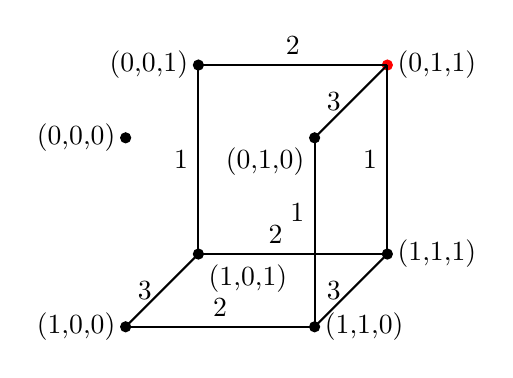
\begin{tikzpicture}[thick,scale=0.2]
	\coordinate[label={180:\text{(1,0,0)}}] (UVL) at (0,0,12);
	\coordinate[label={0:\text{(1,1,0)}}] (UVR) at (12,0,12);
	\coordinate[label={180:\text{(0,0,0)}}] (OVL) at (0,12,12);
	\coordinate[label={-120:\text{(0,1,0)}}] (OVR) at (12,12,12);
	\coordinate[label={-86:\text{(1,0,1)}}] (UHL) at (0,0,0);
	\coordinate[label={0:\text{(1,1,1)}}] (UHR) at (12,0,0);
	\coordinate[label={180:\text{(0,0,1)}}] (OHL) at (0,12,0);
	\coordinate[label={0:\text{(0,1,1)}}] (OHR) at (12,12,0);
	
	\draw[fill=black] (UVL) circle (8pt);
	\draw[fill=black] (UVR) circle (8pt);
	\draw[fill=black] (OVL) circle (8pt);
	\draw[fill=black] (OVR) circle (8pt);
	\draw[fill=black] (UHL) circle (8pt);
	\draw[fill=black] (UHR) circle (8pt);
	\draw[fill=black] (OHL) circle (8pt);
	\filldraw[color=red] (OHR) circle (8pt);
	
	\draw (UVL) -- node[above] {2} (UVR);

	\draw (UVL) -- node[left] {3} (UHL);

	\draw (OVR) -- node[left] {3} (OHR);
	\draw (OVR) -- node[above left] {1} (UVR);
	
	\draw (OHL) -- node[above] {2} (OHR);
	\draw (OHL) -- node[left] {1} (UHL);
	\draw (UHR) -- node[left] {3} (UVR);
	\draw (UHR) -- node[left] {1} (OHR);
	\draw (UHR) -- node[above left] {2} (UHL);
	\end{tikzpicture}
	\caption{Kripke-Modell nach der Ansprache der Königin.}
	\label{nachAnsprache}
\end{figure}

Da es nach der Ansprache das gemeinsame Wissen gibt, dass es mindestens einen untreuen Ehemann in Atlantis gibt, kann der Zustand (0,0,0) von allen Ehefrauen ausgeschlossen werden. Alle Kanten zu (0,0,0) werden entfernt.
Der entscheidende Unterschied zur Ausgangssituation besteht darin, dass es nun Zustände gibt, die von einzelnen Ehefrauen eindeutig identifiziert werden können, von denen also keine Kante mit der Beschriftung ihrer Nummer ausgeht. Dies sind alle Zustände, in denen nur ein Ehemann untreu war.
Der Induktions-Anfang aus Kapitel \ref{motivation} nutzt gerade diese Eigenschaft. Wenn es $n=1$ untreue Ehemänner gibt, so kennt dessen Ehefrau keinen untreuen Ehemann und induziert daher, dass ihr eigener Ehemann untreu gewesen sein muss. Diese Situation kann die betroffene Ehefrau mit keiner anderen verwechseln.\\
Da jede Ehefrau in unserem Fall mindestens einen untreuen Ehemann kennt, geschieht in der ersten Nacht nichts. Am nächsten Tag ergibt sich dann die Situation aus Abbildung \ref{zweiterTag}.

\begin{figure}
	\centering
	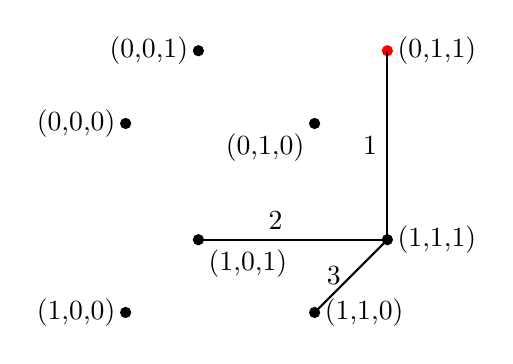
\begin{tikzpicture}[thick,scale=0.2]
	\coordinate[label={180:\text{(1,0,0)}}] (UVL) at (0,0,12);
	\coordinate[label={0:\text{(1,1,0)}}] (UVR) at (12,0,12);
	\coordinate[label={180:\text{(0,0,0)}}] (OVL) at (0,12,12);
	\coordinate[label={-120:\text{(0,1,0)}}] (OVR) at (12,12,12);
	\coordinate[label={-86:\text{(1,0,1)}}] (UHL) at (0,0,0);
	\coordinate[label={0:\text{(1,1,1)}}] (UHR) at (12,0,0);
	\coordinate[label={180:\text{(0,0,1)}}] (OHL) at (0,12,0);
	\coordinate[label={0:\text{(0,1,1)}}] (OHR) at (12,12,0);
	
	\draw[fill=black] (UVL) circle (8pt);
	\draw[fill=black] (UVR) circle (8pt);
	\draw[fill=black] (OVL) circle (8pt);
	\draw[fill=black] (OVR) circle (8pt);
	\draw[fill=black] (UHL) circle (8pt);
	\draw[fill=black] (UHR) circle (8pt);
	\draw[fill=black] (OHL) circle (8pt);
	\filldraw[color=red] (OHR) circle (8pt);	
	
	\draw (UHR) -- node[left] {3} (UVR);
	\draw (UHR) -- node[left] {1} (OHR);
	\draw (UHR) -- node[above left] {2} (UHL);

	\end{tikzpicture}
	\caption{Kripke-Modell nach der ersten Nacht.}
	\label{zweiterTag}
\end{figure}

Da in der ersten Nacht kein Schuss zu hören war, ist es nun gemeinsames Wissen, dass es mindestens zwei untreue Ehemänner gab.
Die zweite und dritte Ehefrau wissen nur von einem untreuen Ehemann und können somit schlussfolgern, dass (0,1,1), der wahre Zustand ist. Beide Ehefrauen erschießen ihren Ehemann, sodass am nächsten Tag auch die erste Ehefrau den korrekten Zustand kennt.

\subsubsection{Visualisierung der Wissensoperatoren}

Um die Äquivalenz der Definitionen für den \textit{jeder weiß}- und den gemeinsames Wissen-Operator aufzuzeigen, betrachten wir noch einmal die Ausgangssituation des \textit{cheating husbands}-Rätsels. 
Die Formel $\Phi$ beschreibe die Eigenschaft, dass es mindestens einen untreuen Ehemann gibt.
In der Ausgangssituation wurde $\Phi$ noch nicht von der Königin bekannt gemacht.
Warum ist $\Phi$ ausgehend vom tatsächlichen Zustand (0,1,1) kein gemeinsames Wissen?\\
Damit $C(\Phi)$ gilt, muss nach der ursprünglichen Definition $E^k(\Phi)$ für alle $k>0$ gelten.
Da jede Ehefrau in diesem Zustand mindestens von einem untreuen Ehemann weiß, gilt $E^1(\Phi)$.
Zwei der drei Ehefrauen wissen nur von einem untreuen Ehemann, sie halten die Welt für möglich, in der dieser Ehemann der einzige untreue war.
Ausgehend von so einer Welt, denken die beiden Ehefrauen weiter, würde die einzige betrogene Ehefrau von keinem untreuen Ehemann wissen.
Im Zustand (0,1,1) weiß somit beispielsweise die dritte Ehefrau nicht, ob die zweite Ehefrau weiß, dass es mindestens einen untreuen Ehemann gibt.
Obwohl jede Ehefrau weiß, dass es mindestens einen untreuen Ehemann gibt, ist diese Information kein gemeinsames Wissen.
Somit gilt in der Ausgangssituation nicht $C(\Phi)$, der Induktionsanfang aus \ref{motivation} greift somit nicht, und es kann nie ein Ehemann erschossen werden.\\
Diese Überlegungen können mit Hilfe der Definitionen zu den \textit{jeder weiß}- und den gemeinsames Wissen-Operator, die k-Erreichbarkeit ausnutzen, leicht am Graphen verifiziert werden.
In jedem Zustand der von (0,1,1) in einem oder keinem Schritt erreichbar ist, gibt es mindestens einen untreuen Ehemann. In zwei Schritten ist allerdings (0,0,0) erreichbar. Somit gilt $E^1(\Phi)$, nicht aber $E^2(\Phi)$, also auch nicht $C(\Phi)$.\\

An dieser Stelle können wir kurz betrachten, warum die Zusätze $^1$ und $^2$ zu den Definitionen von \cite{kshemkalyani2011distributed} sinnvoll sind:
\begin{itemize}
	\item Wird (M,s) $\vDash E^{k}(\phi)$ ohne den Zusatz (oder weniger) definiert, könnte man denken, dass im Zustand (0,0,0) $E^1(\Phi)$ gilt, denn in allen Zuständen, die in genau einem Schritt erreichbar sind, gilt $\Phi$. Dies gilt allerdings offensichtlich nicht, denn jede der drei Ehefrauen hält in diesem Zustand auch den Zustand (0,0,0) selbst für möglich. Technisch gesehen ist (0,0,0) auch in einem Schritt von (0,0,0) erreichbar, denn es existiert eine Folge von Zuständen $s_0$ und $s_1$, wobei $s_0$ = (0,0,0) und $s_1$ = (0,0,0), die für jedes $P_i$ in $\mathcal{K}_i$ enthalten sind. Dies erscheint jedoch recht unintuitiv.
	\item Wird die generelle Erreichbarkeit mit einem $k > 1$ definiert, gibt es ebenso Situationen in denen unintuitive Zustandsfolgen mit dem selben Zustand genutzt werden müssen, um Eigenschaften zu zeigen. So muss in einem Kripke-Modell, in dem nur der Zustand (0,0,0) existiert, die Folge (0,0,0),(0,0,0),(0,0,0) betrachtet werden, wenn man zeigen möchte, dass $\Phi$ nicht gilt.
\end{itemize}
 
 